%%%%%%%%%%%%%%%%%%%%%%%%%%%%%%%%%%%%%%%%%%%%%%%%%%%%%%%%%%%%%%%%%%%%%%%%%%%%%%%%%%
\begin{frame}[fragile]\frametitle{}
\begin{center}
{\Large RAG Framework}
\end{center}
\end{frame}

%%%%%%%%%%%%%%%%%%%%%%%%%%%%%%%%%%%%%%%%%%%%%%%%%%%%%%%%%%%
\begin{frame}[fragile]\frametitle{What is a fine-tuned LLM?}


		\begin{center}
		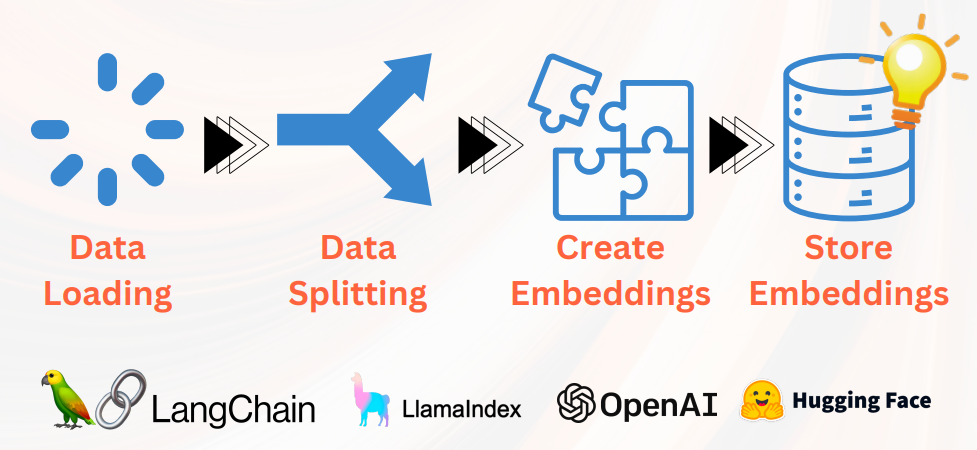
\includegraphics[width=\linewidth,keepaspectratio]{rag15}
		\end{center}

{\tiny (Ref: Knowledge Brain RAG - Abhinav  Kimothi)}

\end{frame}

%%%%%%%%%%%%%%%%%%%%%%%%%%%%%%%%%%%%%%%%%%%%%%%%%%%%%%%%%%%%%%%%%%%%%%%%%%%%%%%%%%
\begin{frame}[fragile]{Loading Data}
    \begin{itemize}
        \item Websites \& HTML pages
        \item Documents like word, pdf etc.
        \item Code in python, java etc.
        \item Data in json, csv etc.
        \item APIs
        \item File Directories
        \item Databases
        \item And many more
    \end{itemize}
\end{frame}

%%%%%%%%%%%%%%%%%%%%%%%%%%%%%%%%%%%%%%%%%%%%%%%%%%%%%%%%%%%%%%%%%%%%%%%%%%%%%%%%%%
\begin{frame}[fragile]{Document Splitting}
    \begin{itemize}
        \item Websites \& HTML pages
        \item Documents like word, pdf etc.
        \item Code in python, java etc.
        \item Data in json, csv etc.
        \item APIs
        \item File Directories
        \item Databases
        \item And many more
    \end{itemize}
\end{frame}


%%%%%%%%%%%%%%%%%%%%%%%%%%%%%%%%%%%%%%%%%%%%%%%%%%%%%%%%%%%%%%%%%%%%%%%%%%%%%%%%%%
\begin{frame}[fragile]{RAG Pipeline Considerations}
    \begin{itemize}
        \item RAG expands non-parametric memory of \#llms.
        \item Indexing pipeline creates a knowledge base for the RAG pipeline.
        \item Crucial step: Splitting documents into manageable chunks (Chunking).
            \begin{itemize}
                \item Large chunks are harder to search; chunking aids in better indexing.
                \item Retrieved context should be significantly smaller than the LLM's context window.
            \end{itemize}
        \item Chunking strategies depend on:
            \begin{itemize}
                \item Nature of the content.
                \item Embedding models chosen.
                \item Length/Complexity of user inputs (context window limitations).
                \item Use Case.
            \end{enumerate}
    \end{itemize}
\end{frame}

%%%%%%%%%%%%%%%%%%%%%%%%%%%%%%%%%%%%%%%%%%%%%%%%%%%%%%%%%%%%%%%%%%%%%%%%%%%%%%%%%%
\begin{frame}[fragile]{Importance of Document Chunking}
  \begin{itemize}
    \item \textbf{Ease of Search:} Larger data chunks are harder to search efficiently, making document splitting crucial for better indexation.
    \item \textbf{Context Window Size:} Large Language Models (LLMs) have finite token limits, necessitating document chunking to fit within the context window.
  \end{itemize}
\end{frame}

%%%%%%%%%%%%%%%%%%%%%%%%%%%%%%%%%%%%%%%%%%%%%%%%%%%%%%%%%%%%%%%%%%%%%%%%%%%%%%%%%%
\begin{frame}[fragile]{Considerations for Chunking Strategies}
  \begin{itemize}
    \item \textbf{Nature of Content:} Adapt chunking strategy based on document length (articles vs. tweets) and the chosen model.
    \item \textbf{Embedding Model:} Choice of embedding model influences the optimal chunking strategy based on performance with specific lengths.
    \item \textbf{User Queries:} Adjust chunking based on expected query length and complexity for improved correlation.
    \item \textbf{Application-Specific Requirements:} Tailor chunking to application needs, considering token limits of downstream models.
  \end{itemize}
\end{frame}

%%%%%%%%%%%%%%%%%%%%%%%%%%%%%%%%%%%%%%%%%%%%%%%%%%%%%%%%%%%%%%%%%%%%%%%%%%%%%%%%%%
\begin{frame}[fragile]{Chunking Methods Overview}
  \begin{itemize}
    \item \textbf{Divide and Merge Approach:} Split text into meaningful units (sentences), merge into larger chunks, and treat them as independent segments.
    \item \textbf{Pre-determined Size and Overlap:} Determine chunk size and specify overlap to maintain contextual continuity between chunks.
  \end{itemize}
\end{frame}

%%%%%%%%%%%%%%%%%%%%%%%%%%%%%%%%%%%%%%%%%%%%%%%%%%%%%%%%%%%%%%%%%%%%%%%%%%%%%%%%%%
\begin{frame}[fragile]{Text Splitting Approaches}
  \begin{itemize}
    \item \textbf{Split by Character:} Divide text based on characters, measuring chunk size by the number of characters.
    \item \textbf{Recursive Split by Character:} Hierarchical splitting using a list of characters for gradual chunking, recommended for generic text.
    \item \textbf{Split by Tokens:} Utilize token limits of LLMs, count tokens while creating chunks, and leverage tokenizers (e.g., Hugging Face Tokenizer).
  \end{itemize}
\end{frame}

%%%%%%%%%%%%%%%%%%%%%%%%%%%%%%%%%%%%%%%%%%%%%%%%%%%%%%%%%%%%%%%%%%%%%%%%%%%%%%%%%%
\begin{frame}[fragile]{Hugging Face Tokenizer}
  \begin{itemize}
    \item \textbf{Tokenization Platform:} Hugging Face is a widely used platform for LLMs, providing access to models along with their tokenizers.
  \end{itemize}
\end{frame}

%%%%%%%%%%%%%%%%%%%%%%%%%%%%%%%%%%%%%%%%%%%%%%%%%%%%%%%%%%%%%%%%%%%%%%%%%%%%%%%%%%
\begin{frame}[fragile]{Specialized Chunking}
  \begin{itemize}
    \item \textbf{Document Structure Honoring:} Consider specific document structures (HTML, Markdown, Latex, code) for preserving context during chunking.
  \end{itemize}
\end{frame}

%%%%%%%%%%%%%%%%%%%%%%%%%%%%%%%%%%%%%%%%%%%%%%%%%%%%%%%%%%%%%%%%%%%%%%%%%%%%%%%%%%
\begin{frame}[fragile]{Things to Keep in Mind}
  \begin{itemize}
    \item \textbf{Data Quality:} Preprocess data for optimal chunk size, removing noise elements like HTML tags.
    \item \textbf{Balance Context and Accuracy:} Find a balance between preserving context and maintaining accuracy in chunking.
    \item \textbf{Test Different Chunk Sizes:} Evaluate and compare performance by creating embeddings for different chunk sizes in the index through queries.
  \end{itemize}
\end{frame}

%%%%%%%%%%%%%%%%%%%%%%%%%%%%%%%%%%%%%%%%%%%%%%%%%%%%%%%%%%%%%%%%%%%%%%%%%%%%%%%%%%
\begin{frame}[fragile]{Embeddings}
  \begin{itemize}
    \item All ML/AI models operate with numerical data.
    \item Embeddings are n-dimensional matrices capturing meaningful relationships in data.
    \item Word embeddings represent words as vectors, a crucial concept for RAG applications.
  \end{itemize}
\end{frame}

%%%%%%%%%%%%%%%%%%%%%%%%%%%%%%%%%%%%%%%%%%%%%%%%%%%%%%%%%%%%%%%%%%%%%%%%%%%%%%%%%%
\begin{frame}[fragile]{Generalization through Transfer Learning}
  \begin{itemize}
    \item Embeddings enable transfer learning, allowing generalization across tasks and domains.
    \item Transfer learning facilitates switching contexts seamlessly.
    \item Popularity of embeddings in ML applications is attributed to this generalization capability.
  \end{itemize}
\end{frame}

%%%%%%%%%%%%%%%%%%%%%%%%%%%%%%%%%%%%%%%%%%%%%%%%%%%%%%%%%%%%%%%%%%%%%%%%%%%%%%%%%%
\begin{frame}[fragile]{Popular Embedding Models}
  \begin{columns}
    \column{0.5\textwidth}
      \begin{itemize}
        \item \textbf{word2vec:}
          \begin{itemize}
            \item Pre-trained word embeddings by Google.
            \item Vector representation of words.
          \end{itemize}
        \item \textbf{GLOVE:}
          \begin{itemize}
            \item Global Vectors model capturing statistics at a global level.
          \end{itemize}
      \end{itemize}
    \column{0.5\textwidth}
      \begin{itemize}
        \item \textbf{fastText:}
          \begin{itemize}
            \item Embeddings built from characters instead of words.
            \item Developed by Facebook's AI research.
          \end{itemize}
        \item \textbf{Elmo:}
          \begin{itemize}
            \item Embeddings from Language Models based on bidirectional LSTM.
          \end{itemize}
        \item \textbf{BERT:}
          \begin{itemize}
            \item Bidirectional Encoder Representations from Transformers.
            \item Transformer-based approach.
          \end{itemize}
      \end{itemize}
  \end{columns}
\end{frame}

%%%%%%%%%%%%%%%%%%%%%%%%%%%%%%%%%%%%%%%%%%%%%%%%%%%%%%%%%%%%%%%%%%%%%%%%%%%%%%%%%%
\begin{frame}[fragile]{Choosing Embeddings}
  \begin{itemize}
    \item \textbf{Landscape Overview:}
      \begin{itemize}
        \item The release of ChatGPT and the LLM Wars increased the development of embedding models.
        \item Evolving standards for evaluating LLMs and embeddings.
      \end{itemize}
    \item \textbf{Use Case Variability:}
      \begin{itemize}
        \item No universal answer to "Which embeddings model to use?"
        \item Some embeddings may perform better for specific use cases (summarization, text generation, classification).
      \end{itemize}
  \end{itemize}
\end{frame}

%%%%%%%%%%%%%%%%%%%%%%%%%%%%%%%%%%%%%%%%%%%%%%%%%%%%%%%%%%%%%%%%%%%%%%%%%%%%%%%%%%
\begin{frame}[fragile]{MTEB Leaderboard}
  \begin{itemize}
    \item \textbf{Hugging Face's MTEB Leaderboard:}
      \begin{itemize}
        \item Evaluates various embedding models across seven use cases.
        \item Use cases include Classification, Clustering, Pair Classification, Reranking, Retrieval, Semantic Textual Similarity (STS), and Summarization.
      \end{itemize}
  \end{itemize}
\end{frame}

%%%%%%%%%%%%%%%%%%%%%%%%%%%%%%%%%%%%%%%%%%%%%%%%%%%%%%%%%%%%%%%%%%%%%%%%%%%%%%%%%%
\begin{frame}[fragile]{Cost Considerations}
  \begin{itemize}
    \item \textbf{OpenAI Models:}
      \begin{itemize}
        \item Significant costs with OpenAI models, especially with large document sets.
        \item Costs depend on the implementation for open-source models.
      \end{itemize}
  \end{itemize}
\end{frame}

%%%%%%%%%%%%%%%%%%%%%%%%%%%%%%%%%%%%%%%%%%%%%%%%%%%%%%%%%%%%%%%%%%%%%%%%%%%%%%%%%%
\begin{frame}[fragile]{Creating Embeddings}
  \begin{itemize}
    \item \textbf{Embedding Creation:}
      \begin{itemize}
        \item After choosing an embedding model, various methods exist for creating embeddings.
        \item Tools like LlamaIndex and LangChain assist in converting documents into vector embeddings.
        \item Directly use services from providers or obtain embeddings from HuggingFace.
      \end{itemize}
  \end{itemize}
\end{frame}

%%%%%%%%%%%%%%%%%%%%%%%%%%%%%%%%%%%%%%%%%%%%%%%%%%%%%%%%%%%%%%%%%%%%%%%%%%%%%%%%%%
\begin{frame}[fragile]{Conclusion}
  \begin{itemize}
    \item Embeddings are essential for RAG applications.
    \item The choice of embeddings depends on use cases, and no one-size-fits-all solution exists.
    \item Continuous evolution in the landscape necessitates staying updated with emerging models and standards.
  \end{itemize}
\end{frame}